\chapter{广度优先搜索}
当题目看不出任何规律,既不能用分治,贪心,也不能用动规时,这时候万能方法——搜索,
就派上用场了。搜索分为广搜和深搜,广搜里面又有普通广搜,双向广搜,A*搜索等。
深搜里面又有普通深搜,回溯法等。

广搜和深搜非常类似(除了在扩展节点这部分不一样),二者有相同的框架,如何表示状态?
如何扩展状态?如何判重?尤其是判重,解决了这个问题,基本上整个问题就解决了。

广度优先搜索算法是按照广度优先的顺序遍历状态空间,一般采用队列实现。

【标记重复以节省重复搜索】
【双向广度优先搜索】
【迭代加深搜索】
【剪枝】
【启发式搜索】通过估价函数进行优化处理,例如最短路径时,$f(x)=dist(x)+h(x,B)$最小的点进行扩展。其中$dist(x)$表示当前已知点到x的最短距离,而$h(x,B)$表示启发函数从x到B得距离。具体过程:每次我们先利用堆找到f值的最小x,让其出堆,然后从它开始拓展新节点。对于x的相邻节点y,如果y还没有被扩展,将其入堆,否则考虑$dist(x)+h(x,B)$,其中$dist(x)$表示边(x,y)的长度,如果这个值小于$dist(y)$则更新$dist(y)$并将其放入堆中。
\section{走迷宫} %%%%%%%%%%%%%%%%%%%%%%%%%%%%%%

\subsubsection{描述}
一个迷宫由一个01矩阵表示,每个单元格要么是空地(用0表示),要
么是障碍物(用1表示)。你的任务是找到一条从入口到出口的最短路径。任何时候都不能在障碍物格子中,也不
能走到迷宫之外。只能横着走或竖着走,不能斜着走。数据保证有唯一解。

\subsubsection{输入}
一个$5 \times 5$的二维数组

\subsubsection{输出}
左上角到右下角的最短路径

\subsubsection{样例输入}
\begin{Code}
0 1 0 0 0
0 1 0 1 0
0 0 0 0 0
0 1 1 1 0
0 0 0 1 0
\end{Code}

\subsubsection{样例输出}
(0, 0)
(1, 0)
(2, 0)
(2, 1)
(2, 2)
(2, 3)
(2, 4)
(3, 4)
(4, 4)

\subsubsection{分析}
既然求的是“最短”,很自然的思路是用BFS。举个例子,在如下图所示的迷宫中,假设
入口是左上角$(0,0)$,我们就从入口开始用BFS遍历迷宫,就可以算出从入口到
所有点的最短路径(如图~\ref{fig:maze}(a)所示),以及这些路径上每个节点的
前驱(如图~\ref{fig:maze}(b)所示)。

\begin{center}
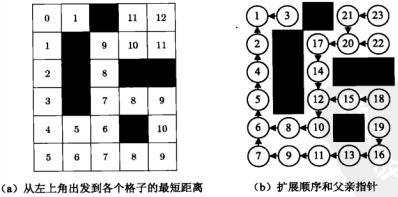
\includegraphics{maze.png}\\
\figcaption{用BFS求迷宫中最短路径}\label{fig:maze}
\end{center}

\subsubsection{代码}
\begin{Codex}[label=maze.c]
/* POJ 3984 迷宫问题, http://poj.org/problem?id=3984 */
#include <cstdio>
#include <cstring>
#include <queue>

const int MAXN = 5;

// 迷宫的行数,列数
int m = MAXN, n = MAXN;
// 迷宫,0表示空地,1表示障碍物
int map[MAXN][MAXN];

// 四个方向
const char name[4] = { 'U', 'R', 'D', 'L' };
const int dx[4] = { -1, 0, 1, 0 }; // 行
const int dy[4] = { 0, 1, 0, -1 }; // 列


typedef struct state_t {
    int data;
    int action;
    int father;
} state_t;

const int STATE_MAX = MAXN * MAXN;  /* 状态总数 */

state_t nodes[STATE_MAX];

int state_hash(const state_t &s);

int state_index(const state_t &s) {
    return state_hash(s);
}

void print_action(const int end) {
    if (nodes[end].father == -1) return;

    print_action(nodes[end].father);
    putchar(name[nodes[end].action]);
}

void print_path(const int end) {
    if (nodes[end].father == -1) {
        printf("(%d, %d)\n", end / n, end % n);
        return;
    }
    print_path(nodes[end].father);
    printf("(%d, %d)\n", end / n, end % n);
}

void hashset_init();

bool hashset_find(const state_t &s);

void hashset_insert(const state_t &s);

void state_extend_init(const state_t &s);

bool state_extend(const state_t &s, state_t &next);

bool state_is_target(const state_t &s);

int bfs(state_t &start) {
    queue<state_t> q;
    hashset_init();

    start.action = -1;
    start.father = -1;

    nodes[state_index(start)] = start;
    hashset_insert(start);
    if (state_is_target(start))
        return state_index(start);
    q.push(start);

    while (!q.empty()) {
        const state_t s = q.front(); q.pop();
        state_t next;

        state_extend_init(s);
        while (state_extend(s, next)) {
            if (state_is_target(next)) {
                return state_index(next);
            }
            q.push(next);
            hashset_insert(next);
        }
    }
    return -1;
}

int main(void) {
    state_t start = {0, -1, -1}; /* 左上角为起点 */
    int end;

    for (int i = 0; i < m; i++) {
        for (int j = 0; j < n; j++) {
            scanf("%d", &map[i][j]);
        }
    }

    end = bfs(start);
    print_path(end);
    return 0;
}

/********** functions implement **************/
/* 存在完美哈希方案 */

const int HASH_CAPACITY = STATE_MAX;
bool visited[HASH_CAPACITY];

int state_hash(const state_t &s) {
    return s.data;
}

void hashset_init() {
    memset(visited, 0, sizeof(visited));
}

bool hashset_find(const state_t &s) {
    return visited[state_hash(s)] == true;
}

void hashset_insert(const state_t &s) {
    visited[state_hash(s)] = true;
}

int action_cur;
#define ACTION_BEGIN 0
#define ACTION_END 4
/** 扩展点,即当前位置 */
int x, y;

void state_extend_init(const state_t &s) {
    action_cur = ACTION_BEGIN;
    x = s.data / n;
    y = s.data % n;
}

bool state_extend(const state_t &s, state_t &next) {
    while(action_cur < ACTION_END) {
        const int nx = x + dx[action_cur];
        const int ny = y + dy[action_cur];

        if (nx >= 0 && nx < m && ny >= 0 && ny < n && !map[nx][ny]) {
            next.data = nx * n + ny;

            if (!hashset_find(next)) { /* 判重 */
                /* 记录路径 */
                next.action = action_cur;
                next.father = state_hash(s);
                nodes[state_index(next)] = next;

                action_cur++;  /* return前别忘了增1 */
                return true;
            }
        }
        action_cur++;
    }
    return false;
}

const state_t END = {24, -1, -1};
bool state_is_target(const state_t &s) {
    return s.data == END.data;
}
\end{Codex}

\subsubsection{相关的题目}
与本题相同的题目:
\begindot
\item 《算法竞赛入门经典》\footnote{刘汝佳,算法竞赛入门经典,清华大学出版社,2009}第108页6.4.2节
\item  POJ 3984 迷宫问题, \myurl{http://poj.org/problem?id=3984}
\myenddot

与本题相似的题目:
\begindot
\item  POJ 2049 Finding Nemo, \myurl{http://poj.org/problem?id=2049}
\myenddot


\section{八数码问题} %%%%%%%%%%%%%%%%%%%%%%%%%%%%%%
\label{subsec:eightDigits}

\subsubsection{描述}
编号为1$\sim$8的8个正方形滑块摆成3行3列,有一个格子空着,如图~\ref{fig:eightDigits}所示。

\begin{center}
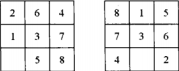
\includegraphics{eight-digits.png}\\
\figcaption{用BFS求迷宫中最短路径}\label{fig:eightDigits}
\end{center}

每次可以把与空格相邻的滑块(有公共边才算相邻)移到空格中,而它原
来的位置就成了新的空格。目标局面固定如下(用$x$表示空格):
\begin{Code}
1 2 3
4 5 6
7 8 x
\end{Code}

给定初始局面,计算出最短的移动路径。

\subsubsection{输入}
用一行表示一个局面,例如下面的这个局面:
\begin{Code}
 1  2  3
 x  4  6
 7  5  8
\end{Code}
可以表示为 1 2 3 x 4 6 7 5 8。 

\subsubsection{输出}
如果有解答,输出一个由四个字母'r','l','u','d'组成的移动路径。
如果没有,输出"unsolvable"。 

\subsubsection{样例输入}
\begin{Code}
2  3  4  1  5  x  7  6  8
\end{Code}

\subsubsection{样例输出}
\begin{Code}
ullddrurdllurdruldr
\end{Code}

\subsubsection{分析}
计算“最短”,很自然的想到BFS。

如何表示一个状态?一个3*3的棋盘,首先可以想到用一个数组\fn{int data[9]}来表示。把每个格子看做是整数的一位的话,可以用一个整数来表示,最大的棋盘87654321x,表示成整数就是876543210,没有超过32位整数的范围。

如何判重?用哈希表,自己实现或者用STL。C++ STL 里有\fn{set}, C++ 11新加入了\fn{unordered_set}。建议先用STL写一个版本,确保主算法正确,然后把\fn{set}(或\fn{unordered_set})替换成自己写的哈希表。

由于本题的特殊性,存在一种完美哈希(perfect hashing)方案。即\textbf{康托展开}。棋盘本身是一个排列,将排列转化为序数,用序数作为hash值。例如,1,2,3 这三个数字的全排列,按字典序,依次为
\begin{Code}
123 -- 0
132 -- 1
213 -- 2
231 -- 3
312 -- 4
321 -- 5
\end{Code}
其中,左侧为排列,右侧为其序数。

此题更优的解法还有双向BFS(见\S \ref{sec:biBFS}),A*算法(见\S \ref{sec:astar})。

\subsubsection{代码}

方案1,完美哈希,使用康托展开。

\begin{Codex}[label=eight_digits_bfs.c]
/* POJ 1077 Eight, http://poj.org/problem?id=1077 */
#include <cstdio>
#include <cstring>
#include <queue>

const int DIGITS = 9; // 棋盘中数字的个数,也是变进制数需要的位数
const int MATRIX_EDGE = 3;       // 棋盘边长

/***** 一些常量 *****/
const int SPACE_NUMBER = 0; // 空格对应着数字 0
// 上下左右四个方向
const int dx[] = {-1, 1, 0, 0};
const int dy[] = {0, 0, -1, 1};
const char name[] = { 'u', 'd', 'l', 'r' };

typedef char int8_t;

/**
 * @strut 状态
 */
typedef struct state_t {
    int8_t data[DIGITS];  /** 状态的数据. */
    int action; /* 由父状态移动到本状态的动作 */
    int father; /* 父状态在nodes[]中的下标,也即父状态的哈希值 */
    int count;  /** 所花费的步骤数(也即路径长度-1) */
} state_t;

// 3x3的棋盘,状态最多有 9!种
const int STATE_MAX = 362880;  /* 状态总数 */

state_t nodes[STATE_MAX+1];

int state_hash(const state_t &s);

int state_index(const state_t &s) {
    return state_hash(s);
}

/**
 * @brief 打印动作序列.
 * @param[in] end 终点状态的哈希值
 * @return 父状态
 */
void print_action(const int end) {
    if (nodes[end].father == -1) return;

    print_action(nodes[end].father);
    putchar(name[nodes[end].action]);
}

void hashset_init();

bool hashset_find(const state_t *s);

void hashset_insert(const state_t *s);

void state_extend_init(const state_t *s);

bool state_extend(const state_t *s, state_t *next);

bool state_is_target(const state_t *s);


int bfs(state_t *start) {
    queue<state_t> q;
    hashset_init();

    start->action = -1;
    start->father = -1;
    start->count = 0;

    nodes[state_index(start)] = *start;
    hashset_insert(start);
    if (state_is_target(start))
        return state_index(start);
    q.push(*start);

    while (!q.empty()) {
        const state_t s = q.front(); q.pop();
        state_t next;

        state_extend_init(&s);
        while (state_extend(&s, &next)) {
            if (state_is_target(&next)) {
                // printf("%d\n", next.count);
                return state_index(&next);
            }
            q.push(next);
            hashset_insert(&next);
        }
    }
    return -1;
}

/**
 * @brief 输入.
 * @return 无
 */
void input(state_t *start) {
    int ch;
    for (int i = 0; i < DIGITS; ++i) {
        do {
            ch = getchar();
        } while ((ch != EOF) && ((ch < '1') || (ch > '8')) && (ch != 'x'));
        if (ch == EOF) return;
        if (ch == 'x') start->data[i] = 0; // x 映射成数字 0
        else           start->data[i] = ch - '0';
    }
}

/** for wikioi 1225 */
void input1(state_t *start) {
    int n;
    scanf("%d", &n);

    /* 将整数转化为棋盘 */
    for(int i = DIGITS-1; i >= 0; i--) {
        start->data[i] = n % 10;
        n /= 10;
    }
}

int main(void) {
    state_t start;
    int end; /* 目标状态在nodes[]中的下标 */
    input(&start);

    end = bfs(&start);

    print_action(end);
    printf("\n");
    return 0;
}

/********** functions implement **************/

/********** 方案1,完美哈希,使用康托展开 **************/

// 9 位变进制数(空格)能表示0到(9!-1)内的所有自然数,恰好有9!个,
// 与状态一一对应,因此可以把状态一一映射到一个9位变进制数

// 9 位变进制数,每个位数的单位,0!~8!
const int fac[] = {40320, 5040, 720, 120, 24, 6, 2, 1, 1};
/* 哈希表容量,要大于状态总数,若存在完美哈希方案,则等于状态总数 */
const int HASH_CAPACITY = STATE_MAX;

bool visited[HASH_CAPACITY];

int state_hash(const state_t *s) {
    int key = 0;
    for (int i = 0; i < DIGITS; i++) {
        int cnt = 0;  /* 逆序数 */
        for (int j = i + 1; j < DIGITS; j++) if (s->data[i] > s->data[j]) cnt++;
        key += fac[i] * cnt;
    }
    return key;
}

void hashset_init() {
    memset(visited, 0, sizeof(visited));
}

bool hashset_find(const state_t *s) {
    return visited[state_hash(s)] == true;
}

void hashset_insert(const state_t *s) {
    visited[state_hash(s)] = true;
}

int action_cur;
#define ACTION_BEGIN 0
#define ACTION_END 4

/* 扩展点,即0的位置 */
int z;

void state_extend_init(const state_t *s) {
    action_cur = ACTION_BEGIN;
    for (z = 0; z < DIGITS; z++) {
        if (s->data[z] == SPACE_NUMBER) {
            break;  // 找 0 的位置
        }
    }
}

bool state_extend(const state_t *s, state_t *next) {
    const int x = z / MATRIX_EDGE; // 行
    const int y = z % MATRIX_EDGE; // 列

    while (action_cur < ACTION_END) {
        const int newx = x + dx[action_cur];
        const int newy = y + dy[action_cur];
        const int newz = newx * MATRIX_EDGE + newy;

        if (newx >= 0 && newx < MATRIX_EDGE && newy >= 0 &&
                newy < MATRIX_EDGE) { // 没有越界
            *next = *s;
            next->data[newz] = SPACE_NUMBER;
            next->data[z] = s->data[newz];
            next->count = s->count + 1;
            if (!hashset_find(next)) { /* 判重 */
                next->action = action_cur;
                next->father = state_hash(s);
                /* 记录路径 */
                nodes[state_index(next)] = *next;
                action_cur++; /* return前别忘了增1 */
                return true;
            }
        }
        action_cur++;
    }
    return false;
}

// 目标状态
const state_t END = {{1, 2, 3, 4, 5, 6, 7, 8, 0}, -1, -1};
// for wikioi 1225
const state_t END1 = {{1, 2, 3, 8, 0, 4, 7, 6, 5}, -1, -1};

bool state_is_target(const state_t *s) {
    return memcmp(s->data, END.data, DIGITS * sizeof(int8_t)) == 0;
}
\end{Codex}

方案2,不知道是否存在完美哈希方案,但能够预估状态个数的上限,用树双亲表示法存储路径,用自己实现的哈希表判重。

\begin{Codex}[label=eight_digits_bfs2.c]
/* POJ 1077 Eight, http://poj.org/problem?id=1077 */
#include <cstdio>
#include <cstring>
#include <queue>
#include <algorithm>

const int DIGITS = 9; // 棋盘中数字的个数,也是变进制数需要的位数
const int MATRIX_EDGE = 3;       // 棋盘边长

/***** 一些常量 *****/
const int SPACE_NUMBER = 0; // 空格对应着数字 0
// 上下左右四个方向
const int dx[] = {-1, 1, 0, 0};
const int dy[] = {0, 0, -1, 1};
const char name[] = { 'u', 'd', 'l', 'r' };

typedef signed char int8_t;

/** 状态 */
struct state_t {
    int8_t data[DIGITS];  /** 状态的数据. */
    int action; /* 由父状态移动到本状态的动作 */
    int index;  /** 本状态在nodes[]中的下标 */
    int father; /** 父状态在nodes[]中的下标 */
    int count;  /** 所花费的步骤数(也即路径长度-1) */
};

// 3x3的棋盘,状态最多有 9!种
const int STATE_MAX = 362880;  /* 状态总数 */

state_t nodes[STATE_MAX+1];
int path_index = 0;

int state_index(const state_t &s) {
    return s.index;
}

/**
 * @brief 打印动作序列.
 * @param[in] end 终点状态的哈希值
 * @return 父状态
 */
void print_action(const int end) {
    if (nodes[end].father == -1) return;

    print_action(nodes[end].father);
    putchar(name[nodes[end].action]);
}

void hashset_init();

bool hashset_find(const state_t &s);

void hashset_insert(const state_t &s);

void state_extend_init(const state_t &s);

bool state_extend(const state_t &s, state_t &next);

bool state_is_target(const state_t &s);

int bfs(state_t &start) {
    queue<state_t> q;
    hashset_init();

    start.action = -1;
    start.index = path_index++;
    start.father = -1;
    start.count = 0;

    nodes[state_index(start)] = start;
    hashset_insert(start);
    if (state_is_target(start))
        return state_index(start);
    q.push(start);

    while (!q.empty()) {
        const state_t s = q.front(); q.pop();
        state_t next;

        state_extend_init(s);
        while (state_extend(s, next)) {
            if (state_is_target(next)) {
                // printf("%d\n", next.count);
                return state_index(next);
            }
            q.push(next);
            hashset_insert(next);
        }
    }
    return -1;
}

/**
 * @brief 输入.
 * @return 无
 */
void input(state_t &start) {
    int ch;
    for (int i = 0; i < DIGITS; ++i) {
        do {
            ch = getchar();
        } while ((ch != EOF) && ((ch < '1') || (ch > '8')) && (ch != 'x'));
        if (ch == EOF) return;
        if (ch == 'x') start.data[i] = 0; // x 映射成数字 0
        else           start.data[i] = ch - '0';
    }
}

/** for wikioi 1225 */
void input1(state_t &start) {
    int n;
    scanf("%d", &n);

    /* 将整数转化为棋盘 */
    for(int i = DIGITS-1; i >= 0; i--) {
        start.data[i] = n % 10;
        n /= 10;
    }
}

int main(void) {
    state_t start;
    int end;
    input(start);

    end = bfs(start);

    print_action(end);
    printf("\n");
    return 0;
}

/********** functions implement **************/

/********** 方案2 不知道完美哈希方案,自己实现哈希表 **************/
/** 哈希表取模的质数,也即哈希桶的个数,越大越好,不过一般小于 HASH_SET_CAPACITY. */
const int PRIME = 99997;

/* 哈希表容量,要大于状态总数 */
const int HASH_SET_CAPACITY = STATE_MAX + 1;

int head[PRIME];
int next[HASH_SET_CAPACITY];

/** 元素的哈希函数  */
int state_hash(const state_t &s) {
    int ret = 0;
    for(int i = 0; i < DIGITS; i++) ret = ret * 10 + s.data[i];
    return ret % PRIME;
}

void hashset_init() {
    fill(head, head + PRIME, -1);
    fill(next, next + PRIME, -1);
}

bool hashset_find(const state_t &s) {
    // 从表头开始查找单链表
    for (int i = head[state_hash(s)]; i != -1; i = next[i]) {
        // 找到了
        if(memcmp(nodes[i].data, s.data,
                DIGITS * sizeof(int8_t)) == 0)
            return true;
    }
    return false;
}

void hashset_insert(const state_t &s) {
    const int h = state_hash(s);
    // 从表头开始查找单链表
    for (int i = head[h]; i != -1; i = next[i]) {
        // 找到了
        if (memcmp(nodes[i].data, s.data,
                DIGITS * sizeof(int8_t)) == 0)
            return;
    }
    next[s.index] = head[h]; /* 插入到首节点前面,头查法 */
    head[h] = s.index;
    return;
}

int action_cur;
#define ACTION_BEGIN 0
#define ACTION_END 4

/* 扩展点,即0的位置 */
int z;

void state_extend_init(const state_t &s) {
    action_cur = ACTION_BEGIN;
    for (z = 0; z < DIGITS; z++) {
        if (s.data[z] == SPACE_NUMBER) {
            break;  // 找 0 的位置
        }
    }
}

bool state_extend(const state_t &s, state_t &next) {
    const int x = z / MATRIX_EDGE; // 行
    const int y = z % MATRIX_EDGE; // 列

    while (action_cur < ACTION_END) {
        const int newx = x + dx[action_cur];
        const int newy = y + dy[action_cur];
        const int newz = newx * MATRIX_EDGE + newy;

        next.count = s.count + 1;
        if (newx >= 0 && newx < MATRIX_EDGE && newy >= 0 &&
                newy < MATRIX_EDGE) { // 没有越界
            next = s;
            next.data[newz] = SPACE_NUMBER;
            next.data[z] = s.data[newz];

            if (!hashset_find(next)) { /* 判重 */
                next.action = action_cur;
                next.index = path_index++;
                next.father = s.index;
                /* 记录路径 */
                nodes[state_index(next)] = next;
                action_cur++; /* return前别忘了增1 */
                return true;
            }
        }
        action_cur++;
    }
    return false;
}

// 目标状态
const state_t END = {{1, 2, 3, 4, 5, 6, 7, 8, 0}, -1, -1};
// for wikioi 1225
const state_t END1 = {{1, 2, 3, 8, 0, 4, 7, 6, 5}, -1, -1};

bool state_is_target(const state_t &s) {
    return memcmp(s.data, END.data, DIGITS * sizeof(int8_t)) == 0;
}
\end{Codex}

方案3,不知道完美哈希方案,但能够预估状态个数的上限制,用树双亲表示法存储路径,用标准库的哈希表判重。

\begin{Codex}[label=eight_digits_bfs3.cpp]
//前面的代码与方案2一摸一样
//...

/********** 方案3 不知道完美哈希方案,使用标准库的哈希表 **************/

// 重载 state_t 的 == 操作符
typedef struct state_t {
    int8_t data[DIGITS];  /** 状态的数据. */
    int action; /* 由父状态移动到本状态的动作 */
    int index;  /** 本状态在nodes[]中的下标 */
    int father; /** 父状态在nodes[]中的下标 */
    int count;  /** 所花费的步骤数(也即路径长度-1) */

    bool operator==(const state_t& other) const {
        return memcmp(data, other.data, DIGITS * sizeof(int8_t)) == 0;
    }
} state_t;

#include <unordered_set>

// 定制一个哈希函数
namespace std {
template<> struct hash<state_t> {
    size_t operator()(const state_t & x) const {
        int i;
        int ret = 0;
        for (i = 0; i < DIGITS; i++)
            ret = ret * 10 + x.data[i];
        return ret;
    }
};
}

unordered_set<state_t> visited;

void hashset_init() {
    visited.clear();
}

bool hashset_find(const state_t &s) {
    return visited.count(s) > 0;
}

void hashset_insert(const state_t &s) {
    visited.insert(s);
}

//...
//后面的代码也与方案2一摸一样
\end{Codex}

\subsubsection{相关的题目}
与本题相同的题目:
\begindot
\item 《算法竞赛入门经典》\footnote{刘汝佳,算法竞赛入门经典,清华大学出版社,2009} 第131页7.5.3节
\item  POJ 1077 Eight, \myurl{http://poj.org/problem?id=1077}
\item  wikioi 1225 八数码难题, \myurl{http://www.wikioi.com/problem/1225/}
\myenddot

与本题相似的题目:
\begindot
\item  POJ 2893 M × N Puzzle, \myurl{http://poj.org/problem?id=2893}
\myenddot


\section{四子连棋} %%%%%%%%%%%%%%%%%%%%%%%%%%%%%%

\subsubsection{描述}
在一个4*4的棋盘上摆放了14颗棋子,其中有7颗白色棋子,7颗黑色棋子,有两个空白地带,任何一颗黑白
棋子都可以向上下左右四个方向移动到相邻的空格,这叫行棋一步,黑白双方交替走棋,任意一方可以先走,
如果某个时刻使得任意一种颜色的棋子形成四个一线(包括斜线),这样的状态为目标棋局。

\subsubsection{输入}
一个4*4的初始棋局,黑棋子用B表示,白棋子用W表示,空格地带用O表示。

\subsubsection{输出}
移动到目标棋局的最少步数。

\subsubsection{样例输入}
\begin{Code}
BWBO
WBWB
BWBW
WBWO
\end{Code}

\subsubsection{样例输出}
\begin{Code}
5
\end{Code}

\subsubsection{分析}
求最少步数,很自然的想到广搜。

如何表示一个状态?用一个二维数组\fn{int board[4][4]}表示,还需要记录该状态是由白子还是黑子移动而导致的,走到该状态已经花费的步数。

如何扩展节点?每一步,从队列弹出一个状态,两个空格都可以向四个方向扩展,把得到的状态入队列。

如何判重?棋盘用二维矩阵存储,用0表示空格,1表示黑色,2表示白色,所以最后可以看成一个16位的三进制数。
用这个数作为棋盘的编码,就可以用来判重了。注意,本题要黑白交替走,所以我们要区分状态是由白子还是黑子移动而导致的。

可以用C++的\fn{map}来判重,
\begin{Code}
/* visited[0]记录白子的历史, visited[1]记录黑子的历史. */
map<int, bool> visited[2];
\end{Code}

也可以开一个大数组当做哈希表,
\begin{Code}
#define HASH_MOD 43036875 /* hash表大小 */
/* visited[0]记录白子的历史, visited[1]记录黑子的历史. */
bool visited[2][HASH_MOD];
\end{Code}

\subsubsection{代码}
\begin{Codex}[label=four_adjacent.cpp]
/** wikioi 1004 四子连棋  , http://www.wikioi.com/problem/1004 */
#include <cstdio>
#include <cstring>
#include <queue>

#define LEN 4   /* 边长 */

/* 右,左,上,下(左下角为坐标原点)*/
const int dx[] = { 1, -1, 0, 0 };
const int dy[] = { 0, 0, 1, -1 };


/**
 * @strut 状态
 */
typedef struct state_t {
    // 状态的数据
    int board[LEN][LEN]; /* 棋局,1表示黑子,2表示白子,0表示空白 */
    int color; /* 本状态是由白子还是黑子移动而导致的 */
    int count;  /** 所花费的步骤数(也即路径长度-1),求路径长度时需要 */
} state_t;

void hashset_init();

bool hashset_find(const state_t &s);

void hashset_insert(const state_t &s);

void state_extend_init(const state_t &s);

bool state_extend(const state_t &s, state_t &next);

bool state_is_target(const state_t &s);

void bfs(state_t &start) {
    queue<state_t> q;
    hashset_init();

    start.count = 0;
    start.color = 1;

    hashset_insert(start);
    q.push(start);

    start.color = 2;

    hashset_insert(start); // 千万别忘记了标记此处的访问记录
    if (state_is_target(start)) /* 如果起点就是终点,返回 */
        return;
    q.push(start);

    while (!q.empty()) {
        const state_t s = q.front(); q.pop();
        state_t next;

        state_extend_init(s);
        while (state_extend(s, next)) {
            if (state_is_target(next)) {
                printf("%d\n", next.count);
                return;
            }
            q.push(next);
            hashset_insert(next);
        }
    }
}

int main() {
    char s[LEN + 1];
    state_t start;

    for (int i = 0; i < LEN; i++) {
        scanf("%s", s);
        for (int j = 0; j < LEN; j++) {
            if (s[j] == 'B') start.board[i][j] = 1;
            else if (s[j] == 'W') start.board[i][j] = 2;
            else start.board[i][j] = 0;
        }
    }

    bfs(start);
    return 0;
}

/************ functions implement ************/

/* 哈希表容量,要大于状态总数,若存在完美哈希方案,则等于状态总数 */
#define HASH_CAPACITY 43036875

/** 哈希表,标记状态是否已访问过。
 * visited[0]记录白子的历史,visited[1]记录黑子的历史.
 */
bool visited[2][HASH_CAPACITY];

#define RADIX 3 /* 三进制 */

/**
 * @brief 计算状态的哈希值。
 * 棋盘用二维矩阵存储,用0表示空格,1表示黑色,2表示白色,所以最后可以看成
 * 一个16位的三进制数。最大为
 * 2222
 * 2221
 * 1111
 * 1100
 * 值为 43036875。
 * @return 棋盘所表示的三进制数转化为十进制数
 */
//TODO:共C16 7×C9 2个状态,用类似康托的方法储存
int state_hash(const state_t &s) {
    int ret = 0;

    for (int i = 0; i < LEN; i++) {
        for (int j = 0; j < LEN; j++) {
            ret = ret * RADIX + s.board[i][j];
        }
    }
    return ret;
}

void hashset_init() {
    fill(visited[0], visited[0] + HASH_CAPACITY, false);
    fill(visited[1], visited[1] + HASH_CAPACITY, false);
}

bool hashset_find(const state_t &s) {
    return visited[s.color - 1][state_hash(s)] == true;
}

void hashset_insert(const state_t &s) {
    visited[s.color - 1][state_hash(s)] = true;
}

/* 扩展的时候,先定空格,再定方向 */
/* 记录当前方向,例如action_cur[0]记录了第一个空格,当前在扩展哪个方向
 */
int action_cur[2];
#define ACTION_BEGIN 0
#define ACTION_END 4

typedef struct point_t {
    int x, y;
} point_t;

/* 记录当前在扩展哪一个空格,值为0或1 */
int space_cur;
/* 两个空格的位置 */
point_t extend_pos[2];

void state_extend_init(const state_t &s) {
    action_cur[0] = ACTION_BEGIN;
    action_cur[1] = ACTION_BEGIN;
    space_cur = 0;

    int k = 0;
    // 寻找两个空白的格子的位置
    for (int i = 0; i < LEN; i++) {
        for (int j = 0; j < LEN; j++) {
            if (s.board[i][j] == 0) {
                extend_pos[k].x = i;
                extend_pos[k].y = j;
                k++;
            }
        }
    }
}

bool state_extend(const state_t &s, state_t &next) {
    for (int i = 0; i < 2; i++) { /* 先第一个空格,再第二个空格 */
        while (action_cur[i] < ACTION_END) {
            const int x = extend_pos[i].x;
            const int y = extend_pos[i].y;
            int nextx = x + dx[action_cur[i]];
            int nexty = y + dy[action_cur[i]];
            next = s;
            next.count = s.count + 1;
            next.color = 3 - s.color;

            if (nextx >= 0 && nextx < LEN && nexty >= 0 && nexty < LEN
                    /* 必须黑白交替走 */
                    && next.color == s.board[nextx][nexty]) {
                /* swap */
                {
                    int temp = next.board[x][y];
                    next.board[x][y] = next.board[nextx][nexty];
                    next.board[nextx][nexty] = temp;
                }

                if (!hashset_find(next)) { /* 判重 */
                    action_cur[i]++; /* return前别忘了增1 */
                    return true;
                }
            }
            action_cur[i]++;
        }
    }
    return false;
}

bool state_is_target(const state_t &s) {
    for (int i = 0; i < LEN; i++) {  /* 逐行检查 */
        int flag = 1;  /* 某一行全是同一颜色 */
        for (int j = 1; j < LEN; j++)
            if (s.board[i][j - 1] != s.board[i][j])
                flag = 0;
        if (flag)
            return 1;
    }
    for (int j = 0; j < LEN; j++) { //逐列检查
        int flag = 1;  /* 某一行全是同一颜色 */
        for (int i = 1; i < LEN; i++)
            if (s.board[i][j] != s.board[i - 1][j]) flag = 0;
        if (flag) return 1;
    }
    /* 斜线 */
    if (s.board[0][0] == s.board[1][1] && s.board[1][1] == s.board[2][2]
            && s.board[2][2] == s.board[3][3])
        return 1;
    if (s.board[0][3] == s.board[1][2] && s.board[1][2] == s.board[2][1]
            && s.board[2][1] == s.board[3][0])
        return 1;
    return 0;
}
\end{Codex}

\subsubsection{相关的题目}
与本题相同的题目:
\begindot
\item  wikioi 1004 四子连棋, \myurl{http://www.wikioi.com/problem/1004/}
\myenddot

与本题相似的题目:
\begindot
\item  None
\myenddot


\section{双向BFS} %%%%%%%%%%%%%%%%%%%%%%%%%%%%%%
\label{sec:biBFS}


\subsection{八数码问题}
题目见 \S \ref{subsec:eightDigits}。

\subsubsection{代码}

\begin{Codex}[label=eight_digits_bibfs.c]

\end{Codex}


\section{A*算法} %%%%%%%%%%%%%%%%%%%%%%%%%%%%%%
\label{sec:astar}

\textbf{A*算法 = 宽搜 + 优先队列}

将广搜模板(见第\S \ref{sec:bfs-template}节)中的队列改为优先队列,设计好当前状态距离目标状态的预估距离$h()$,就变成了A*算法!

\subsection{八数码问题}
题目见 \S \ref{subsec:eightDigits}。

\subsubsection{代码}
\begin{Codex}[label=eight_digits_astar.c]
/** POJ 1077 Eight, http://poj.org/problem?id=1077
 简单解释几个要点,便于理解代码.
1. 怎么判断是否有解?只要计算出的逆序个数总和为奇数,该数据必然无解
2. 如何判断某一状态是否到过?本题存在一种完美哈希方案,即用康托展开。
        详见 http://128kj.iteye.com/blog/1699795
3.使用优先队列,即堆,加速挑选最优值。
4.函数 g=此状态在搜索树中已经走过的路径的节点数.
5.估价函数 h ,采用曼哈顿距离, 见代码 calcH 函数。曼哈顿距离的定义是,
 假设有两个点(x1,y1),(x2,y2),则曼哈顿距离L1=|x1-x2| + |y1-y2|
 */
#include <cstdio>
#include <cstring>
#include <cmath>
#include <queue>

#define DIGITS 9 // 棋盘中数字的个数,也是变进制数需要的位数
#define     MATRIX_EDGE 3       // 棋盘边长
#define RADIX 10

/***** 一些常量 *****/
const int SPACE_NUMBER = 0; // 空格对应着数字 0
// 上下左右四个方向
const int dx[] = {-1, 1, 0, 0};
const int dy[] = {0, 0, -1, 1};
const char name[] = { 'u', 'd', 'l', 'r' };

// 目标状态
const int GOAL = 123456780;
// 每个数字在棋盘中的位置,例如0,在(2,2)=8这个位置上
int GOAL_POS[DIGITS];


/** 状态 */
struct state_t {
    int board;  /** 状态的数据,即棋局. */
    int action; /* 由父状态移动到本状态的动作 */
    int father; /* 父状态在nodes[]中的下标,也即父状态的哈希值 */
    int count;  /** 所花费的步骤数(也即路径长度-1),作为g */
    int h; /** 距离目标状态的估算距离 */

    bool operator>(const state_t &other) const {
        // priority_queue 默认是大根堆,反一下,就是小根堆了
        return (count + h) > (other.count + other.h);
    }
};

// 3x3的棋盘,状态最多有 9!种
#define STATE_MAX 362880  /* 状态总数 */

state_t nodes[STATE_MAX+1];

int state_hash(const state_t &s);

int state_index(const state_t &s) {
    return state_hash(s);
}

/**
 * @brief 打印动作序列.
 * @param[in] end 终点状态的哈希值
 * @return 父状态
 */
void print_action(const int end) {
    if (nodes[end].father == -1) return;

    print_action(nodes[end].father);
    putchar(name[nodes[end].action]);
}

void hashset_init();

bool hashset_find(const state_t &s);

void hashset_insert(const state_t &s);

void state_extend_init(const state_t &s);

bool state_extend(const state_t &s, state_t &next);

bool state_is_target(const state_t &s);

/**
 * 距离目标状态的估算距离h。
 * @param s 状态
 * @return h
 */
static int state_get_h(const state_t &state) {
    int h = 0;
    int s = state.board;

    for (int i = DIGITS - 1; i >= 0; --i) {
        const int p = s % RADIX;
        s /= RADIX;
        /* 曼哈顿距离 */
        h += abs((float)(i / MATRIX_EDGE - GOAL_POS[p] / MATRIX_EDGE)) +
                abs((float)(i % MATRIX_EDGE - GOAL_POS[p] % MATRIX_EDGE));
    }
    return h;
}

/* 计算 GOAL_POS */
static void calc_goal_pos() {
    int cur = GOAL;
    for (int i = DIGITS-1; i >= 0 ; i--) {
        int digit = cur % RADIX;
        GOAL_POS[digit] = i;
        cur /= RADIX;
    }
}

int bfs(state_t &start) {
    priority_queue<state_t, vector<state_t>,
                                 greater<state_t> > q;
    calc_goal_pos();
    hashset_init();

    start.action = -1;
    start.father = -1;
    start.count = 0;
    start.h = state_get_h(start);

    nodes[state_index(start)] = start;
    hashset_insert(start);
    if (state_is_target(start))
        return state_index(start);
    q.push(start);

    while (!q.empty()) {
        const state_t s = q.top(); q.pop();
        //const state_t s = q.front(); q.pop();
        state_t next;

        state_extend_init(s);
        while (state_extend(s, next)) {
            if (state_is_target(next)) {
                // printf("%d\n", next.count);
                return state_index(next);
            }
            q.push(next);
            hashset_insert(next);
        }
    }
    return -1;
}

static void int_to_board(int n, int board[DIGITS]) {
    for (int i = DIGITS - 1; i >= 0; i--) {
        board[i] = n % RADIX;
        n /= RADIX;
    }
}

static int board_to_int(const int board[DIGITS]) {
    int s = 0;
    for (int i = 0; i < DIGITS; i++)
        s = s * RADIX + board[i];
    return s;
}

/**
 * @brief 输入.
 * @return 无
 */
void input(state_t &start) {
    int ch;
    int board[DIGITS];
    for (int i = 0; i < DIGITS; ++i) {
        do {
            ch = getchar();
        } while ((ch != EOF) && ((ch < '1') || (ch > '8')) && (ch != 'x'));
        if (ch == EOF) return;
        if (ch == 'x') board[i] = 0; // x 映射成数字 0
        else           board[i] = ch - '0';
    }
    start.board = board_to_int(board);
}

/** for wikioi 1225 */
void input1(state_t &start) {
    scanf("%d", &start.board);
}

/**
 * 计算一个排列的逆序数,0 除外.
 */
static int inversion_count(int permutation) {
    int d[DIGITS];
    int c = 0; // 逆序数

    for(int i = DIGITS - 1; i >=0; i--) {
        d[i] = permutation % RADIX;
        permutation /= RADIX;
    }

    for (int i = 1; i < DIGITS; i++)  if (d[i] != SPACE_NUMBER) {
        for (int j = 0; j < i; j++) {
            if(d[j] != SPACE_NUMBER) {
                if (d[j] > d[i]) {
                    c++;
                }
            }
        }
    }
    return c;
}

/**
 * 判断是否有解.
 *
 * 求出除0之外所有数字的逆序数之和,也就是每个数字后面比它小的数字的个数的和,
 * 称为这个状态的逆序。
 *
 * 若起始状态和目标状态的逆序数奇偶性相同,则可相互到达,否则不可相互到达。
 *
 * @param s 目标状态
 * @return 1表示有解,0表示无解
 */
static int solvable(const int s) {
    return (inversion_count(s) + inversion_count(GOAL)) % 2 == 0;
}

int main(void) {
    state_t start;
    int end; /* 目标状态在nodes[]中的下标 */
    input(start);

    if (!solvable(start.board)) return 0;

    end = bfs(start);

    print_action(end);
    printf("\n");
    return 0;
}

/********** functions implement **************/

/********** 方案1,完美哈希,使用康托展开 **************/

// 9 位变进制数(空格)能表示0到(9!-1)内的所有自然数,恰好有9!个,
// 与状态一一对应,因此可以把状态一一映射到一个9位变进制数

// 9 位变进制数,每个位数的单位,0!~8!
const int fac[] = {40320, 5040, 720, 120, 24, 6, 2, 1, 1};
/* 哈希表容量,要大于状态总数,若存在完美哈希方案,则等于状态总数 */
#define HASH_CAPACITY STATE_MAX

bool visited[HASH_CAPACITY];

/**
 * @brief 计算状态的hash值,这里用康托展开,是完美哈希.
 * @param[in] s 当前状态
 * @return 序数,作为hash值
 */
int state_hash(const state_t &state) {
    int board[DIGITS];
    int key = 0;

    int_to_board(state.board, board);

    for (int i = 0; i < DIGITS; i++) {
        int c = 0; // 逆序数
        for (int j = i + 1; j < DIGITS; j++) {
            if(board[j] < board[i]) {
                c++;
            }
        }
        key += c * fac[i];
    }

    return key;
}

void hashset_init() {
    fill(visited, visited + HASH_CAPACITY, false);
}

bool hashset_find(const state_t &s) {
    return visited[state_hash(s)] == true;
}

void hashset_insert(const state_t &s) {
    visited[state_hash(s)] = true;
}

int action_cur;
#define ACTION_BEGIN 0
#define ACTION_END 4

/* 扩展点,即0的位置 */
int z;
int board[DIGITS];  /* 棋盘,暂存数据 */

void state_extend_init(const state_t &s) {
    action_cur = ACTION_BEGIN;

    int_to_board(s.board, board);
    for (z = 0; z < DIGITS; z++) {
        if (board[z] == SPACE_NUMBER) {
            break;  // 找 0 的位置
        }
    }
}

bool state_extend(const state_t &s, state_t &next) {
    const int x = z / MATRIX_EDGE; // 行
    const int y = z % MATRIX_EDGE; // 列

    while (action_cur < ACTION_END) {
        const int newx = x + dx[action_cur];
        const int newy = y + dy[action_cur];
        const int newz = newx * MATRIX_EDGE + newy;

        if (newx >= 0 && newx < MATRIX_EDGE && newy >= 0 &&
                newy < MATRIX_EDGE) { // 没有越界
            board[z] = board[newz];
            board[newz] = SPACE_NUMBER;
            next = s;
            next.board = board_to_int(board);
            board[newz] = board[z]; /* 恢复s的棋盘 */
            board[z] = SPACE_NUMBER;

            next.count = s.count + 1;
            next.h = state_get_h(next);
            if (!hashset_find(next)) { /* 判重 */
                next.action = action_cur;
                next.father = state_index(s);
                /* 记录路径 */
                nodes[state_index(next)] = next;
                action_cur++; /* return前别忘了增1 */
                return true;
            }
        }
        action_cur++;
    }
    return false;
}

// 目标状态
const state_t END = {123456780, -1, -1};
// for wikioi 1225
const state_t END1 = {123804765, -1, -1};

bool state_is_target(const state_t &s) {
    return s.board == END.board;
}
\end{Codex}


\section{小结} %%%%%%%%%%%%%%%%%%%%%%%%%%%%%%
\label{sec:bfs-template}


\subsection{适用场景}

\textbf{输入数据}:没什么特征,不像深搜,需要有“递归”的性质。如果是树或者图,概率更大。

\textbf{状态转换图}:树或者图。

\textbf{求解目标}:求最短。


\subsection{思考的步骤}
\begin{enumerate}
\item 是求路径长度,还是路径本身(或动作序列)?
    \begin{enumerate}
    \item 如果是求路径长度,则状态里面要存路径长度
    \item 如果是求路径本身或动作序列
        \begin{enumerate}
            \item 要用一棵树存储宽搜过程中的路径
            \item 是否可以预估状态个数的上限?能够预估状态总数,则开一个大数组,用树的双亲表示法;如果不能预估状态总数,则要使用一棵通用的树。这一步也是第4步的必要不充分条件。
        \end{enumerate}
    \end{enumerate}

\item 如何表示状态?即一个状态需要存储哪些些必要的数据,才能够完整提供如何扩展到下一步状态的所有信息。一般记录当前位置或整体局面。

\item 如何扩展状态?这一步跟第2步相关。状态里记录的数据不同,扩展方法就不同。对于固定不变的数据结构(一般题目直接给出,作为输入数据),如二叉树,图等,扩展方法很简单,直接往下一层走,对于隐式图,要先在第1步里想清楚状态所带的数据,想清楚了这点,那如何扩展就很简单了。

\item 关于判重,状态是否存在完美哈希方案?即将状态一一映射到整数,互相之间不会冲突。
    \begin{enumerate}
    \item 如果不存在,则需要使用通用的哈希表(自己实现或用标准库,例如\fn{unordered_set})来判重;自己实现哈希表的话,如果能够预估状态个数的上限,则可以开两个数组,head和next,表示哈希表,参考第 \S \ref{subsec:eightDigits}节方案2。
    \item 如果存在,则可以开一个大布尔数组,作为哈希表来判重,且此时可以精确计算出状态总数,而不仅仅是预估上限。
    \end{enumerate}

\item 目标状态是否已知?如果题目已经给出了目标状态,可以带来很大便利,这时候可以从起始状态出发,正向广搜;也可以从目标状态出发,逆向广搜;也可以同时出发,双向广搜。
\end{enumerate}


\subsection{代码模板}
广搜需要一个队列,用于一层一层扩展,一个hashset,用于判重,一棵树(只求长度时不需要),用于存储整棵树。

对于队列,如果用纯C,需要造一个队列轮子;如果用C++,可以用\fn{queue},也可以把\fn{vector}当做队列使用。当求长度时,有两种做法:
\begin{enumerate}
\item 只用一个队列,但在状态结构体\fn{state_t}里增加一个整数字段\fn{step},表示走到当前状态用了多少步,当碰到目标状态,直接输出\fn{step}即可。这个方案,可以很方便的变成A*算法,把队列换成优先队列即可。
\item 用两个队列,\fn{current, next},分别表示当前层次和下一层,另设一个全局整数\fn{level},表示层数(也即路径长度),当碰到目标状态,输出\fn{level}即可。这个方案,状态可以少一个字段,节省内存。
\end{enumerate}

对于hashset,如果有完美哈希方案,用布尔数组(\fn{bool visited[STATE_MAX]}或\fn{vector<bool> visited(STATE_MAX, false)})来表示;如果没有,可以用STL里的\fn{set}或\fn{unordered_set}。

对于树,如果用STL,可以用\fn{unordered_map<state_t, state_t > father}表示一颗树,代码非常简洁。如果能够预估状态总数的上限(设为STATE_MAX),可以用数组(\fn{state_t nodes[STATE_MAX]}),即树的双亲表示法来表示树,效率更高,当然,需要写更多代码。


C++风格的模板。
\begin{Codex}[label=bfs_template1.cpp]
/**
 * @brief 反向生成路径.
 * @param[in] father 树
 * @param[in] target 目标节点
 * @return 从起点到target的路径
 */
template<typename state_t>
vector<state_t> gen_path(const unordered_map<state_t, state_t> &father,
        const state_t &target) {
    vector<state_t> path;
    path.push_back(target);

    state_t cur = target;
    while (father.find(cur) != father.end()) {
        cur = father.at(cur);
        path.push_back(cur);
    }
    reverse(path.begin(), path.end());

    return path;
}

/**
 * @brief 广搜.
 * @param[in] state_t 状态,如整数,字符串,一维数组等
 * @param[in] start 起点
 * @param[in] state_is_target 判断状态是否是目标的函数
 * @param[in] state_extend 状态扩展函数
 * @return 从起点到目标状态的一条最短路径
 */
template<typename state_t>
vector<state_t> bfs(state_t &start, bool (*state_is_target)(const state_t&),
        vector<state_t>(*state_extend)(const state_t&,
                unordered_set<string> &visited)) {
    queue<state_t> next, current; // 当前层,下一层
    unordered_set<state_t> visited; // 判重
    unordered_map<state_t, state_t> father;

    int level = 0;  // 层次
    bool found = false;
    state_t target;

    current.push(start);
    visited.insert(start);
    while (!current.empty() && !found) {
        ++level;
        while (!current.empty() && !found) {
            const state_t state = current.front();
            current.pop();
            vector<state_t> new_states = state_extend(state, visited);
            for (auto iter = new_states.begin();
                    iter != new_states.end() && ! found; ++iter) {
                const state_t new_state(*iter);

                if (state_is_target(new_state)) {
                    found = true; //找到了
                    target = new_state;
                    father[new_state] = state;
                    break;
                }

                next.push(new_state);
                // visited.insert(new_state); 必须放到 state_extend()里
                father[new_state] = state;
            }
        }
        swap(next, current); //!!! 交换两个队列
    }

    if (found) {
        return gen_path(father, target);
        //return level + 1;
    } else {
        return vector<state_t>();
        //return 0;
    }
}
\end{Codex}

C风格的模板。
\begin{Codex}[label=bfs_template2.cpp]
#include <cstdio>
#include <cstring>

/***** 输入数据,用全局变量存放 *****/
...
/*
例如
int m = MAXN, n = MAXN;  // 迷宫的行数,列数
// 迷宫,0表示空地,1表示障碍物
int map[MAXN][MAXN];  // 迷宫,0表示空地,1表示障碍物
 */

/***** 一些常量 *****/
...
/* 例如
// 四个方向
const char name[4] = { 'U', 'R', 'D', 'L' };
const int dx[4] = { -1, 0, 1, 0 }; // 行
const int dy[4] = { 0, 1, 0, -1 }; // 列
*/

/** 状态 */
struct state_t {
    ... data1;  /** 状态的数据,可以有多个字段. */
    ... data2;  /** 状态的数据,可以有多个字段. */
    int action; /** 由父状态移动到本状态的动作,求动作序列时需要. */
    int index;  /** 本状态在nodes[]中的下标,求路径和动作序列时需要。
                    如果存在完美哈希,则不需要本字段(此时将
                   状态的哈希值作为下标,而哈希值可以直接计算出) */
    int father; /** 父状态在nodes[]中的下标,求路径或动作序列时需要 */
    int count;  /** 所花费的步骤数(也即路径长度-1),求路径长度时需要 */
};

/********** 如果题目要求输出路径或动作序列,则需要下面的变量和函数 ***********/

const int STATE_MAX ...  /* 状态总数 */
/**
 * 记录动作序列,树的双亲表示法.
 * 如果不能预估状态个数的上限,则不能用数组,要用通用树
 * 一般此时会有完美哈希方案,开一个大数组存储每个状态的动作,下标就是状态的哈希值
 * 其实一般用不了这么大的数组,广搜很很快就会结束
 */
state_t nodes[STATE_MAX];
int path_index = 0;  /** 每出现一个新状态,就增1,将状态存到该位置,
                         如果有完美哈希方案,则不需要该变量. */

/**
 * @brief 返回状态在nodes[]中的下标.
 * 
 * 起点状态没有父亲和动作为-1,因为它没有父状态,也就没有所谓的从父节点到它的动作。
 * @param[in] s 状态
 * @return 状态在nodes[]中的下标
 */
int state_index(const state& s) {
    /* 如果有完美哈希方案 */
    return state_hash(s);
    /* 否则 */
    return s.index;
}

/**
 * @brief 打印动作序列.
 * 如果有完美哈希方案,状态的哈希值就是下标。
 * 起点状态没有父亲和动作为-1,因为它没有父状态,也就没有所谓的从父节点到它的动作。
 * @param[in] end 终点状态的下标
 * @return 父状态
 */
void print_action(const int end) {
    if (nodes[end].father == -1) return;

    print_action(nodes[end].father);
    putchar(name[nodes[end].action]);
}

/**
 * @brief 打印坐标序列.
 * 如果有完美哈希方案,状态的哈希值就是下标。
 * 起点状态没有父亲和动作为-1,因为它没有父状态,也就没有所谓的从父节点到它的动作。
 * @param[in] end 终点状态的哈希值
 * @return 父状态
 */
void print_path(const int end) {
    if (nodes[end].father == -1) {
        printf("(%d, %d)\n", end / n, end % n);
        return;
    }
    print_path(nodes[end].father);
    printf("(%d, %d)\n", end / n, end % n);
}

/********** 如果题目要求输出路径或动作序列,则需要上面的变量和函数 ***********/

/** 初始化查找表. */
void hashset_init();

/**
 * @brief 状态判重.
 * 一般用哈希表(set::unordered_set),如果存在完美哈希,则用数组
 * @param[in] s 状态
 * @return 已经访问过,返回true,否则false
 */
bool hashset_find(const state_t &s);

/**
 * @brief 标记该状态已经被访问
 * @param[in] s 状态
 * @return 无
 */
void hashset_insert(const state_t &s);

/**
 * @brief 扩展第一个状态.
 * @param[in] s 状态
 * @param[out] next 第一个状态
 * @return 如果还有下一个状态,返回true,否则返回false
 */
void state_extend_init(const state_t &s);

/**
 * @brief 扩展下一个状态.
 * @param[in] s 状态
 * @param[out] next 下一个状态
 * @return 如果还有下一个状态,返回true,否则返回false
 */
bool state_extend(const state_t &s, state_t &next);

/**
 * @brief 判断状态是否为目标.
 * @param[in] s 状态
 * @return 如果已经达到目标状态,返回true,否则false
 */
bool state_is_target(const state_t &s);

/*
 * @brief 广搜
 *
 * @param[in] x 入口的x坐标
 * @param[in] y 入口的y坐标
 * @return 目标状态在nodes[]中的下标,如果不需要求路径,则声明为 void
 */
int bfs(state_t &start) {
    queue<state_t> q;
    hashset_init();

    start.action = -1;   /* 起点状态没有动作 */
    start.index = path_index++;
    start.father = -1;   /* 起点状态没有父状态 */
    start.count = 0;

    nodes[state_index(start)] = start;
    hashset_insert(start); // 千万别忘记了标记此处的访问记录
    if (state_is_target(start)) /* 如果起点就是终点,返回 */
        return state_index(start);
    q.push(start);

    while (!q.empty()) {
        const state_t s = q.front(); q.pop();
        state_t next;

        state_extend_init(&s);
        while (state_extend(&s, &next)) {
            if (state_is_target(&next)) {
                // printf("%d\n", next.count);
                return state_index(next);
            }
            q.push(next);
            hashset_insert(&next);
        }
    }
    return -1;
}

int main(void) {
    state_t start;
    int end; /* 目标状态在nodes[]中的下标 */
    input(start);

    end = bfs(start);

    print_action(end);
    printf("\n");
    print_path(end);
    return 0;
}

/************ functions implement ************/

/** 哈希表取模的质数,也即哈希桶的个数,越大越好,不过一般小于 HASH_SET_CAPACITY. */
#define PRIME ...  /* 99997 */

/* 哈希表容量,要大于状态总数,若存在完美哈希方案,则等于状态总数 */
#define HASH_CAPACITY STATE_MAX

/** 哈希表,标记状态是否已访问过。
 * 如果存在完美哈希方案,则用数组作为哈希表,否则用unordered_set
 */
... visited
// 例如 bool visited[HASH_CAPACITY];
// 或者
// int head[PRIME];
// int next[HASH_CAPACITY];

/** 计算状态的哈希值.
 * 哈希值应该只依赖state_t的数据字段。
 */
int state_hash(const state_t &s) {
    ...
}

void hashset_init() {
    /* 如果是数组 */
    memset(visited, 0, sizeof(visited));
    /* 如果是 unordered_set */
    visited.clear();
}

bool hashset_find(const state_t &s) {
    /* 如果是数组 */
    return visited[state_hash(s)] == true;
    /* 如果是 unordered_set */
    return visited.count(s) > 0;
}

void hashset_insert(const state_t &s) {
    /* 如果是数组 */
    visited[state_hash(s)] = true;
    /* 如果是 unordered_set */
    visited.insert(s);
}

/** 扩展节点时,记录当前到了什么哪一步.
 * 是state_extend_init()和state_extend()的共享变量
 */
int action_cur;
/* 动作的范围 */
#define ACTION_BEGIN ...
#define ACTION_END ...

/* 扩展点的位置,是 state_extend_init()和state_extend()的共享变量 */
int extend_pos;

void state_extend_init(const state_t &s) {
    action_cur = ACTION_BEGIN;
    extend_pos = // 根据 s 进行计算
}

bool state_extend(const state_t &s, state_t &next) {
    // extract values from s
    value1 = ...
    value2 = ...
    while(action_cur < ACTION_END) {
        // apply action_cur to values
        value1 = ...
        value2 = ...
        next.count = s.count + 1;
        if (values are valid) {
            // assign new values to next's data fields
            next.data1 = value1
            next.data2 = value2

            if (!hashset_find(next)) { /* 判重 */
                next.action = action_cur;
                next.index = path_index++;
                next.father = state_index(s);
                /* 记录路径 */
                nodes[state_index(next)] = next;
                action_cur++;  /* return前别忘了增1 */
                return true;
            }
        }
        action_cur++;
    }
    return false;
}

// 目标状态
const state_t END = {..., 0};

bool state_is_target(const state_t &s) {
    ...
    /* 例如 return memcmp(s.data, END.data, xx * sizeof(yy) == 0; */
    /* 例如 return s.data == END.data; */
}
\end{Codex}


\section{Word Ladder} %%%%%%%%%%%%%%%%%%%%%%%%%%%%%%
\label{sec:word-ladder}


\subsubsection{描述}
Given two words (start and end), and a dictionary, find the length of shortest transformation sequence from start to end, such that:
\begindot
\item Only one letter can be changed at a time
\item Each intermediate word must exist in the dictionary
\myenddot

For example, Given:

\begin{Code}
	start = "hit"
	end = "cog"
	dict = ["hot","dot","dog","lot","log"]
\end{Code}
As one shortest transformation is \code{"hit" -> "hot" -> "dot" -> "dog" -> "cog"}, return its length $5$.

Note:
\begindot
\item Return 0 if there is no such transformation sequence.
\item All words have the same length.
\item All words contain only lowercase alphabetic characters.
\myenddot


\subsubsection{分析}


\subsubsection{代码}
\begin{Code}
	//LeetCode, Word Ladder
	// 时间复杂度O(n),空间复杂度O(n)
	class Solution {
		public:
		int ladderLength(const string& start, const string &end,
		const unordered_set<string> &dict) {
			queue<string> current, next;    // 当前层,下一层
			unordered_set<string> visited;  // 判重
			
			int level = 0;  // 层次
			bool found = false;
			
			auto state_is_target = [&](const string &s) {return s == end;};
			auto state_extend = [&](const string &s) {
				vector<string> result;
				
				for (size_t i = 0; i < s.size(); ++i) {
					string new_word(s);
					for (char c = 'a'; c <= 'z'; c++) {
						if (c == new_word[i]) continue;
						
						swap(c, new_word[i]);
						
						if ((dict.count(new_word) > 0 || new_word == end) &&
						!visited.count(new_word)) {
							result.push_back(new_word);
							visited.insert(new_word);
						}
						swap(c, new_word[i]); // 恢复该单词
					}
				}
				
				return result;
			};
			
			current.push(start);
			while (!current.empty() && !found) {
				++level;
				while (!current.empty() && !found) {
					const string str = current.front();
					current.pop();
					
					const auto& new_states = state_extend(str);
					for (const auto& state : new_states) {
						next.push(state);
						if (state_is_target(state)) {
							found = true; //找到了
							break;
						}
					}
				}
				swap(next, current);
			}
			if (found) return level + 1;
			else return 0;
		}
	};
\end{Code}


\subsubsection{相关题目}

\begindot
\item Word Ladder II,见 \S \ref{sec:word-ladder-ii}
\myenddot


\section{Word Ladder II} %%%%%%%%%%%%%%%%%%%%%%%%%%%%%%
\label{sec:word-ladder-ii}


\subsubsection{描述}
Given two words (start and end), and a dictionary, find all shortest transformation sequence(s) from start to end, such that:
\begindot
\item Only one letter can be changed at a time
\item Each intermediate word must exist in the dictionary
\myenddot

For example, Given:
\begin{Code}
	start = "hit"
	end = "cog"
	dict = ["hot","dot","dog","lot","log"]
\end{Code}
Return
\begin{Code}
	[
	["hit","hot","dot","dog","cog"],
	["hit","hot","lot","log","cog"]
	]
\end{Code}

Note:
\begindot
\item All words have the same length.
\item All words contain only lowercase alphabetic characters.
\myenddot


\subsubsection{分析}
跟 Word Ladder比,这题是求路径本身,不是路径长度,也是BFS,略微麻烦点。

这题跟普通的广搜有很大的不同,就是要输出所有路径,因此在记录前驱和判重地方与普通广搜略有不同。


\subsubsection{代码}

\begin{Code}
	//LeetCode, Word Ladder II
	// 时间复杂度O(n),空间复杂度O(n)
	class Solution {
		public:
		vector<vector<string> > findLadders(string start, string end,
		const unordered_set<string> &dict) {
			unordered_set<string> current, next;  // 当前层,下一层,用集合是为了去重
			unordered_set<string> visited; // 判重
			unordered_map<string, vector<string> > father; // 树
			
			bool found = false;
			
			auto state_is_target = [&](const string &s) {return s == end;};
			auto state_extend = [&](const string &s) {
				unordered_set<string> result;
				
				for (size_t i = 0; i < s.size(); ++i) {
					string new_word(s);
					for (char c = 'a'; c <= 'z'; c++) {
						if (c == new_word[i]) continue;
						
						swap(c, new_word[i]);
						
						if ((dict.count(new_word) > 0|| new_word == end) &&
						!visited.count(new_word)) {
							result.insert(new_word);
						}
						swap(c, new_word[i]); // 恢复该单词
					}
				}
				
				return result;
			};
			
			current.insert(start);
			while (!current.empty() && !found) {
				// 先将本层全部置为已访问,防止同层之间互相指向
				for (const auto& word : current)
				visited.insert(word);
				for (const auto& word : current) {
					const auto new_states = state_extend(word);
					for (const auto &state : new_states) {
						if (state_is_target(state)) found = true;
						next.insert(state);
						father[state].push_back(word);
						// visited.insert(state); // 移动到最上面了
					}
				}
				
				current.clear();
				swap(current, next);
			}
			vector<vector<string> > result;
			if (found) {
				vector<string> path;
				gen_path(father, path, start, end, result);
			}
			return result;
		}
		private:
		void gen_path(unordered_map<string, vector<string> > &father,
		vector<string> &path, const string &start, const string &word,
		vector<vector<string> > &result) {
			path.push_back(word);
			if (word == start) {
				result.push_back(path);
				reverse(result.back().begin(), result.back().end());
			} else {
			for (const auto& f : father[word]) {
				gen_path(father, path, start, f, result);
			}
		}
		path.pop_back();
	}
};
\end{Code}


\subsubsection{相关题目}

\begindot
\item Word Ladder,见 \S \ref{sec:word-ladder}
\myenddot


\section{Surrounded Regions} %%%%%%%%%%%%%%%%%%%%%%%%%%%%%%
\label{sec:surrounded-regions}


\subsubsection{描述}
Given a 2D board containing \fn{'X'} and \fn{'O'}, capture all regions surrounded by \fn{'X'}.

A region is captured by flipping all \fn{'O'}s into \fn{'X'}s in that surrounded region .

For example,
\begin{Code}
	X X X X
	X O O X
	X X O X
	X O X X
\end{Code}

After running your function, the board should be:
\begin{Code}
	X X X X
	X X X X
	X X X X
	X O X X
\end{Code}


\subsubsection{分析}
广搜。从上下左右四个边界往里走,凡是能碰到的\fn{'O'},都是跟边界接壤的,应该保留。


\subsubsection{代码}
\begin{Code}
	// LeetCode, Surrounded Regions
	// BFS,时间复杂度O(n),空间复杂度O(n)
	class Solution {
		public:
		void solve(vector<vector<char>> &board) {
			if (board.empty()) return;
			
			const int m = board.size();
			const int n = board[0].size();
			for (int i = 0; i < n; i++) {
				bfs(board, 0, i);
				bfs(board, m - 1, i);
			}
			for (int j = 1; j < m - 1; j++) {
				bfs(board, j, 0);
				bfs(board, j, n - 1);
			}
			for (int i = 0; i < m; i++)
			for (int j = 0; j < n; j++)
			if (board[i][j] == 'O')
			board[i][j] = 'X';
			else if (board[i][j] == '+')
			board[i][j] = 'O';
		}
		private:
		void bfs(vector<vector<char>> &board, int i, int j) {
			typedef pair<int, int> state_t;
			queue<state_t> q;
			const int m = board.size();
			const int n = board[0].size();
			
			auto is_valid = [&](const state_t &s) {
				const int x = s.first;
				const int y = s.second;
				if (x < 0 || x >= m || y < 0 || y >= n || board[x][y] != 'O')
				return false;
				return true;
			};
			
			auto state_extend = [&](const state_t &s) {
				vector<state_t> result;
				const int x = s.first;
				const int y = s.second;
				// 上下左右
				const state_t new_states[4] = {{x-1,y}, {x+1,y},
					{x,y-1}, {x,y+1}};
				for (int k = 0; k < 4;  ++k) {
					if (is_valid(new_states[k])) {
						// 既有标记功能又有去重功能
						board[new_states[k].first][new_states[k].second] = '+';
						result.push_back(new_states[k]);
					}
				}
				
				return result;
			};
			
			state_t start = { i, j };
			if (is_valid(start)) {
				board[i][j] = '+';
				q.push(start);
			}
			while (!q.empty()) {
				auto cur = q.front();
				q.pop();
				auto new_states = state_extend(cur);
				for (auto s : new_states) q.push(s);
			}
		}
	};
\end{Code}


\subsubsection{相关题目}

\begindot
\item 无
\myenddot


\section{小结} %%%%%%%%%%%%%%%%%%%%%%%%%%%%%%
\label{sec:bfs-template}


\subsection{适用场景}

\textbf{输入数据}:没什么特征,不像深搜,需要有“递归”的性质。如果是树或者图,概率更大。

\textbf{状态转换图}:树或者图。

\textbf{求解目标}:求最短。


\subsection{思考的步骤}
\begin{enumerate}
	\item 是求路径长度,还是路径本身(或动作序列)?
	\begin{enumerate}
		\item 如果是求路径长度,则状态里面要存路径长度(或双队列+一个全局变量)
		\item 如果是求路径本身或动作序列
		\begin{enumerate}
			\item 要用一棵树存储宽搜过程中的路径
			\item 是否可以预估状态个数的上限?能够预估状态总数,则开一个大数组,用树的双亲表示法;如果不能预估状态总数,则要使用一棵通用的树。这一步也是第4步的必要不充分条件。
		\end{enumerate}
	\end{enumerate}
	
	\item 如何表示状态?即一个状态需要存储哪些些必要的数据,才能够完整提供如何扩展到下一步状态的所有信息。一般记录当前位置或整体局面。
	
	\item 
	如何扩展状态?这一步跟第2步相关。状态里记录的数据不同,扩展方法就不同。对于固定不变的数据结构(一般题目直接给出,作为输入数据),如二叉树,图等,扩展方法很简单,直接往下一层走,对于隐式图,要先在第1步里想清楚状态所带的数据,想清楚了这点,那如何扩展就很简单了。
	
	\item 关于判重,状态是否存在完美哈希方案?即将状态一一映射到整数,互相之间不会冲突。
	\begin{enumerate}
		\item 如果不存在,则需要使用通用的哈希表(自己实现或用标准库,例如\fn{unordered_set})来判重;自己实现哈希表的话,如果能够预估状态个数的上限,则可以开两个数组,head和next,表示哈希表,参考第 \S 
		\ref{subsec:eightDigits}节方案2。
		\item 如果存在,则可以开一个大布尔数组,作为哈希表来判重,且此时可以精确计算出状态总数,而不仅仅是预估上限。
	\end{enumerate}
	
	\item 目标状态是否已知?如果题目已经给出了目标状态,可以带来很大便利,这时候可以从起始状态出发,正向广搜;也可以从目标状态出发,逆向广搜;也可以同时出发,双向广搜。
\end{enumerate}


\subsection{代码模板}
广搜需要一个队列,用于一层一层扩展,一个hashset,用于判重,一棵树(只求长度时不需要),用于存储整棵树。

对于队列,可以用\fn{queue},也可以把\fn{vector}当做队列使用。当求长度时,有两种做法:
\begin{enumerate}
	\item 只用一个队列,但在状态结构体\fn{state_t}里增加一个整数字段\fn{step},表示走到当前状态用了多少步,当碰到目标状态,直接输出\fn{step}即可。这个方案,可以很方便的变成A*算法,把队列换成优先队列即可。
	\item 用两个队列,\fn{current, next},分别表示当前层次和下一层,另设一个全局整数\fn{level},表示层数(也即路径长度),当碰到目标状态,输出\fn{level}即可。这个方案,状态可以少一个字段,节省内存。
\end{enumerate}

对于hashset,如果有完美哈希方案,用布尔数组(\fn{bool visited[STATE_MAX]}或\fn{vector<bool> visited(STATE_MAX, false)})来表示;如果没有,可以用STL里的\fn{set}或\fn{unordered_set}。

对于树,如果用STL,可以用\fn{unordered_map<state_t, state_t > father}表示一颗树,代码非常简洁。如果能够预估状态总数的上限(设为STATE_MAX),可以用数组(\fn{state_t 
nodes[STATE_MAX]}),即树的双亲表示法来表示树,效率更高,当然,需要写更多代码。


\subsubsection{双队列的写法}
\begin{Codex}[label=bfs_template1.cpp]
	/** 状态 */
	struct state_t {
		int data1;  /** 状态的数据,可以有多个字段. */
		int data2;  /** 状态的数据,可以有多个字段. */
		// dataN;   /** 其他字段 */
		int action; /** 由父状态移动到本状态的动作,求动作序列时需要. */
		int count;  /** 所花费的步骤数(也即路径长度-1),求路径长度时需要;
		不过,采用双队列时不需要本字段,只需全局设一个整数 */
		bool operator==(const state_t &other) const {
			return true;  // 根据具体问题实现
		}
	};
	
	// 定义hash函数
	
	// 方法1:模板特化,当hash函数只需要状态本身,不需要其他数据时,用这个方法比较简洁
	namespace std {
		template<> struct hash<state_t> {
			size_t operator()(const state_t & x) const {
				return 0; // 根据具体问题实现
			}
		};
	}
	
	// 方法2:函数对象,如果hash函数需要运行时数据,则用这种方法
	class Hasher {
		public:
		Hasher(int _m) : m(_m) {};
		size_t operator()(const state_t &s) const {
			return 0; // 根据具体问题实现
		}
		private:
		int m; // 存放外面传入的数据
	};
	
	
	/**
	* @brief 反向生成路径.
	* @param[in] father 树
	* @param[in] target 目标节点
	* @return 从起点到target的路径
	*/
	template<typename state_t>
	vector<state_t> gen_path(const unordered_map<state_t, state_t> &father,
	const state_t &target) {
		vector<state_t> path;
		path.push_back(target);
		
		for (state_t cur = target; father.find(cur) != father.end(); 
		cur = father.at(cur))
		path.push_back(cur);
		
		reverse(path.begin(), path.end());
		
		return path;
	}
	
	/**
	* @brief 广搜.
	* @param[in] state_t 状态,如整数,字符串,一维数组等
	* @param[in] start 起点
	* @param[in] grid 输入数据
	* @return 从起点到目标状态的一条最短路径
	*/
	template<typename state_t>
	vector<state_t> bfs(const state_t &start, const vector<vector<int>> &grid) {
		queue<state_t> next, current; // 当前层,下一层
		unordered_set<state_t> visited; // 判重
		unordered_map<state_t, state_t> father; // 树
		
		int level = 0;  // 层次
		bool found = false; // 是否找到目标
		state_t target; // 符合条件的目标状态
		
		// 判断当前状态是否为所求目标
		auto state_is_target = [&](const state_t &s) {return true; };
		// 扩展当前状态
		auto state_extend = [&](const state_t &s) {
			vector<state_t> result;
			// ...
			return result;
		};
		
		current.push(start);
		visited.insert(start);
		while (!current.empty() && !found) {
			++level;
			while (!current.empty() && !found) {
				const state_t state = current.front();
				current.pop();
				vector<state_t> new_states = state_extend(state);
				for (auto iter = new_states.cbegin();
				iter != new_states.cend() && ! found; ++iter) {
					const state_t new_state(*iter);
					
					if (state_is_target(new_state)) {
						found = true; //找到了
						target = new_state;
						father[new_state] = state;
						break;
					}
					
					next.push(new_state);
					// visited.insert(new_state); 必须放到 state_extend()里
					father[new_state] = state;
				}
			}
			swap(next, current); //!!! 交换两个队列
		}
		
		if (found) {
			return gen_path(father, target);
			//return level + 1;
		} else {
		return vector<state_t>();
		//return 0;
	}
}
\end{Codex}


\subsubsection{只用一个队列的写法}
双队列的写法,当求路径长度时,不需要在状态里设置一个\fn{count}字段记录路径长度,只需全局设置一个整数\fn{level},比较节省内存;只用一个队列的写法,当求路径长度时,需要在状态里设置一个\fn{count}字段,不过,这种写法有一个好处
 —— 可以很容易的变为A*算法,把\fn{queue}替换为\fn{priority_queue}即可。

\begin{Codex}[label=bfs_template2.cpp]
	// 与模板1相同的部分,不再重复
	// ...
	
	/**
	* @brief 广搜.
	* @param[in] state_t 状态,如整数,字符串,一维数组等
	* @param[in] start 起点
	* @param[in] grid 输入数据
	* @return 从起点到目标状态的一条最短路径
	*/
	template<typename state_t>
	vector<state_t> bfs(state_t &start, const vector<vector<int>> &grid) {
		queue<state_t> q; // 队列
		unordered_set<state_t> visited; // 判重
		unordered_map<state_t, state_t> father; // 树
		
		int level = 0;  // 层次
		bool found = false; // 是否找到目标
		state_t target; // 符合条件的目标状态
		
		// 判断当前状态是否为所求目标
		auto state_is_target = [&](const state_t &s) {return true; };
		// 扩展当前状态
		auto state_extend = [&](const state_t &s) {
			vector<state_t> result;
			// ...
			return result;
		};
		
		start.count = 0;
		q.push(start);
		visited.insert(start);
		while (!q.empty() && !found) {
			const state_t state = q.front();
			q.pop();
			vector<state_t> new_states = state_extend(state);
			for (auto iter = new_states.cbegin();
			iter != new_states.cend() && ! found; ++iter) {
				const state_t new_state(*iter);
				
				if (state_is_target(new_state)) {
					found = true; //找到了
					target = new_state;
					father[new_state] = state;
					break;
				}
				
				q.push(new_state);
				// visited.insert(new_state); 必须放到 state_extend()里
				father[new_state] = state;
			}
		}
		
		if (found) {
			return gen_path(father, target);
			//return level + 1;
		} else {
		return vector<state_t>();
		//return 0;
	}
}
\end{Codex}